\section[Question 4]{Question 4}
\textit{Air pollution exhibits significant geospatial variation across the globe. Investigate if
there is an association in your sample between pm10\_concentration and who\_region
[pick a single year in which to investigate the association]. }

\subsection{Question 4.a}
\textit{Plot an appropriate figure/graph to visualise the relationship between these
two variables. } \\

\noindent Figure \ref{fig:q4_box_pm10_region} shows a box and whiskers plot to show the spread of points between the six WHO regions for 2020.

\begin{figure}[H]
    \centering
    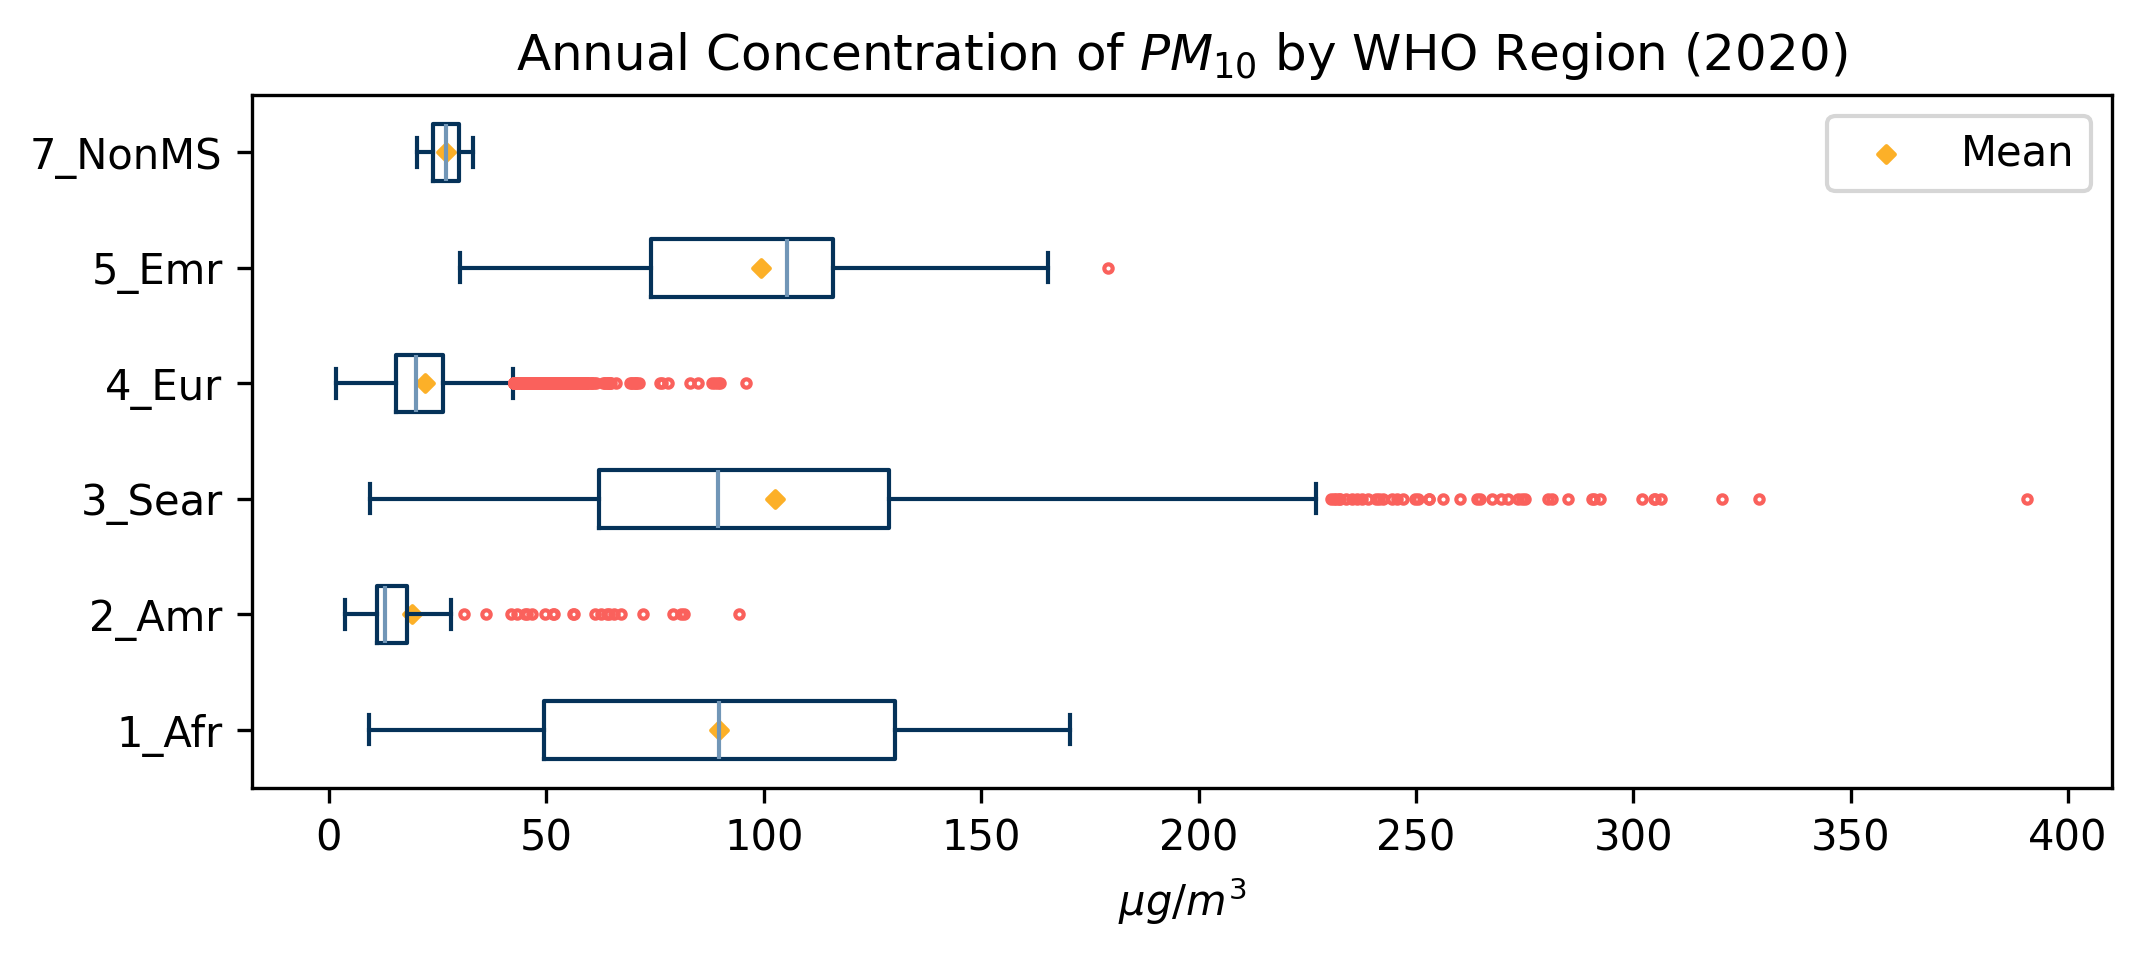
\includegraphics[width=0.8\textwidth]{img/q4_box_pm10_region.png}
    \caption{$PM_{10}$ concentration by WHO region - 2020.}
    \label{fig:q4_box_pm10_region}
\end{figure}

\subsection{Question 4.b}
\textit{Select an appropriate statistical test to test if there is a difference in pm10\_concentration
by who\_region (if in doubt consult the flow charts on Amathuba).
How many groups are being compared and are they paired or independent
groups? Check the assumptions of your chosen statistical test. Report your decisions
on the validity of the assumptions for your chosen statistical test. Justify your
decisions. Report the name of the final test you choose to run.}\\

\noindent Six independent groups are being compared (`1\_Afr', `2\_Amr', `3\_Sear', `4\_Eur', `5\_Emr', `7\_NonMS'). The groups are independent because the $PM_{10}$ concentrations in each region are not related to each other. 

\noindent The data are not normally distributed, as indicated by the Shapiro-Wilk test results. Therefore, the Kruskal-Wallis test (non-parametric alternative of ANOVA) was chosen to compare the median $PM_{10}$ concentrations across the different WHO regions. 


\subsection{Question 4.c}
\textit{Run your chosen test, report the p-value and use your sample data to report
on the direction and magnitude of the effect (use the test results and refer to
your figure from 3a) }

\noindent The Kruskal-Wallis test was used to determine if there is a difference in $PM_{10}$ concentration across the six WHO regions. 


\begin{itemize}
    \item $H_0$: Mean $PM_{10}$ concentration is the same accross all six WHO regions.
    \item $H_A$: Mean $PM_{10}$ concentration is not the same accross all six WHO regions.
\end{itemize}
% The code used to determine the Kruskal-Wallis test is shown in Listing \ref{lst:pm10region}. 

\noindent The Kruskal-Wallis test yielded a $p$-value of 0.00 ($p < 0.05$). Thus, we reject $H_0$ and conclude that there is a difference in $PM_{10}$ concentration means between the six WHO regions. The mean $PM_{10}$ concentration by region is represented by the yellow dots in Figure \ref{fig:q4_box_pm10_region}. 

% \begin{lstlisting}[caption={Python code to evaluate $PM_{10}$ concentration accross six WHO regions}, label={lst:pm10region}]
%     from scipy.stats import kruskal
   
%     statistic, p_value = kruskal(*data_by_region)

% \end{lstlisting}


\newpage